\documentclass[border=1pt]{standalone}
\usepackage{tikz}
\usetikzlibrary{arrows.meta}

\begin{document}
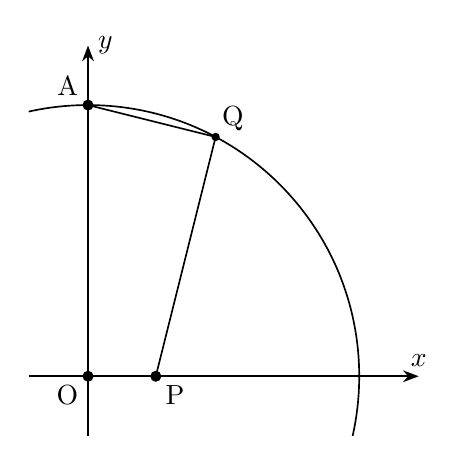
\begin{tikzpicture}

    % パラメータの定義
    \pgfmathsetmacro{\X}{4.2}
    \pgfmathsetmacro{\Y}{\X}
    \pgfmathsetmacro{\r}{0.82*\X}
    \pgfmathsetmacro{\d}{0.18*\X}
    \pgfmathsetmacro{\px}{\r/4}
    \pgfmathsetmacro{\qx}{\r*8/17}
    \pgfmathsetmacro{\qy}{(\r^2-\qx^2)^0.5}

    \coordinate (O) at (0,0);
    \coordinate (A) at (0,\r);
    \coordinate (P) at (\px,0);
    \coordinate (Q) at (\qx,\qy);

    % 軸を描画
    \draw[-Stealth,semithick] (-\d,0) -- (\X,0) node[above] {$x$};
    \draw[-Stealth,semithick] (0,-\d) -- (0,\Y) node[right] {$y$};

    % 円を描画
    \begin{scope}
        \clip (-\d,-\d) rectangle (\X,\Y);
        \draw [semithick] (0,0) circle [radius=\r];
    \end{scope}
    
    % 点の描画
    \fill (O) circle (2pt) node[below left] {O};
    \fill (A) circle (2pt) node[above left] {A};
    \fill (P) circle (2pt) node[below right] {P};
    \fill (Q) circle (1.5pt) node[above right,outer sep=-1pt] {Q};

    % 直線の描画
    \draw[semithick] (A) -- (Q);
    \draw[semithick] (P) -- (Q);

\end{tikzpicture}
\end{document}
